\documentclass{beamer}
\beamertemplatenavigationsymbolsempty
\usetheme{Ilmenau}
\usecolortheme{beaver}
%\usepackage[utf8]{inputenc}
\usepackage[english]{babel}
\parindent=0.pt
\usepackage{amsmath}
\usepackage{graphicx}
\usepackage{verbatim}
\usepackage{tikz}
\usepackage{csquotes}
\usepackage{tabularx}
\usepackage{caption}
\usepackage[backend=biber,
style=phys,
citestyle=authoryear
]{biblatex}
\addbibresource{Biblio.bib} 
\usepackage[export]{adjustbox}
\usefonttheme[onlymath]{serif}
\newcommand{\R}{\mathbb{R}}
\renewcommand{\qedsymbol}{\includegraphics[width=0.6in, right]{QED Gregory.png}}


\title{A Fine-Grained Analysis of XGBoost Predicting $T_c$}
\author{Daniel Briseno}

  \begin{document}
  \frame{\titlepage}
  
  
  
  %%%%%%%%%%%%%%%%%%%%% Begin Presentation%%%%%%%%%%%%%%%%%%%%
  
  \begin{frame}{Introduction}
      \begin{figure}
          \centering
          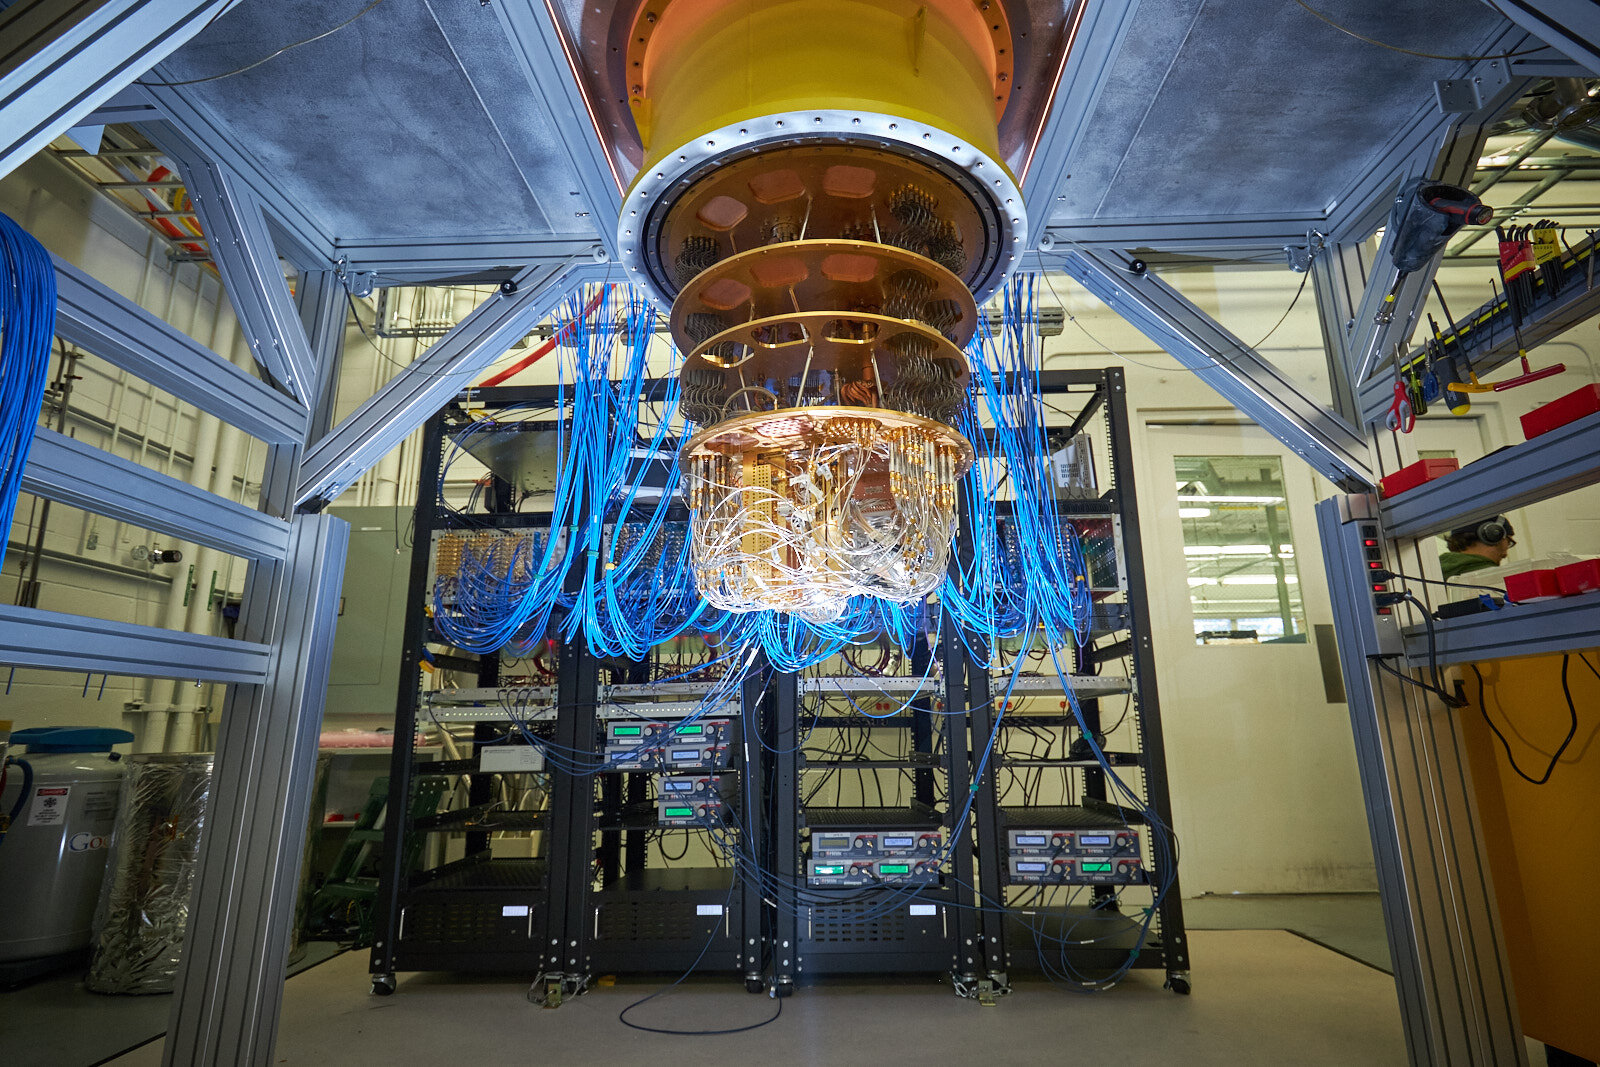
\includegraphics[width = \linewidth]{Google_qc.jpg}
          \caption{Google Quantum Computer}
          \label{fig:my_label}
      \end{figure}
  \end{frame}
  
  \begin{frame}{Introduction}
      \begin{block}{Data-driven $T_c$ Prediction}
        \begin{itemize}
            \item No good physical model for $T_c$
            \item Previous attempts at data-driven $T_c$ prediction focus prediction on small subset of superconductors.(\cite{owolabi_estimation_2015})(\cite{stanev_machine_2018})
            \item XGBoost gradient-boosted decision tree ML algorithm provides $T_c$ prediction for more general class of Superconductors (\cite{hamidieh_data-driven_2018}).
        \end{itemize}
      \end{block}
  \end{frame}
  
  \begin{frame}{Introduction}
    \begin{block}{Principle Questions Motivating Analysis}
      \begin{enumerate}
          \item How well does XGBoost perform at predicting $T_c$ across the true $T_c$ quartiles?
          \item How well does XGBoost perform at the same task across the predicted $T_c$ quartiles?
      \end{enumerate}
    \end{block}
  \end{frame}
  
  \begin{frame}{Introduction}
  \begin{block}{The Data}
    Set of 21263 superconductors, with features defined by summary statistics of the atomic properties for the elements they contain.
  \end{block}
  \begin{table}[h]
     \centering
     \tiny
     \begin{tabularx}{\linewidth}{X X X}
          \hline
          Variable & Units & Description\\
          \hline
        Atomic Mass &Atomic mass units (AMU) &Total proton and neutron rest masses\\
        First Ionization Energy &Kilo-Joules per mole (kJ/mol)&Energy required to remove a valence electron\\
        Atomic Radius & Picometer (pm) &Calculated atomic radius\\
        Density&Kilograms per meters cubed (kg/m3)&Density at standard temperature and pressure\\
        Electron Affinity &Kilo-Joules per mole (kJ/mol) &Energy required to add an electron to a neutral atom\\
        Fusion Heat &Kilo-Joules per mole (kJ/mol) &Energy to change from solid to liquid without temperature change\\
        Thermal Conductivity &Watts per meter-Kelvin (W/(m K)) &Thermal conductivity coefficient $\kappa$\\
        Valence &No units &Typical number of chemical bonds formed by the element\\
        \hline
     \end{tabularx}
     \caption{Elemental properties used to define features used by XGboost to predict $T_c$. }
     \label{tab:elemental_properties}
 \end{table}
  \end{frame}
  
  \begin{frame}{Introduction}
       \begin{figure}
     \centering
     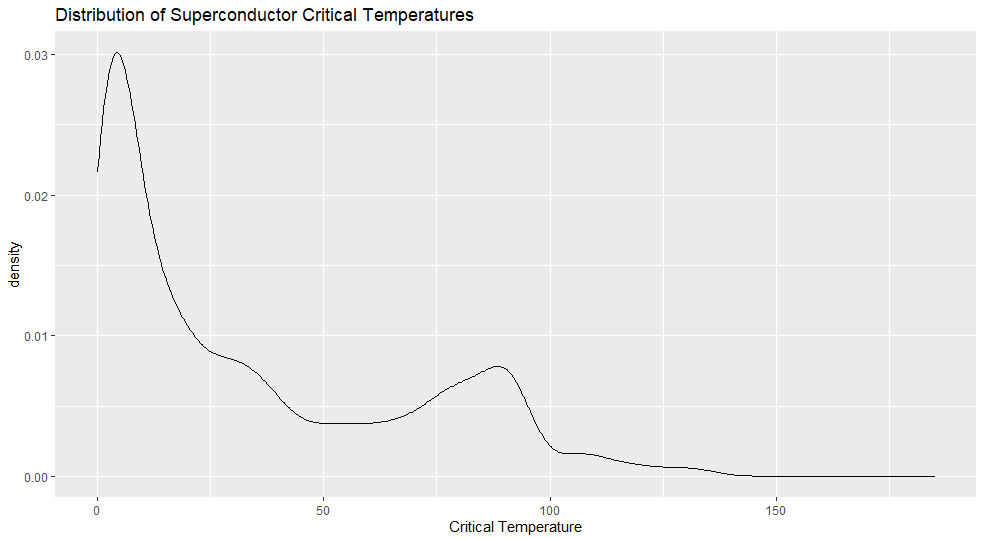
\includegraphics[width=\linewidth]{Tc_dist.png}
     \caption{Density plot of $T_c$ values for all superconductors in dataset.}
     \label{fig:Tc_density}
 \end{figure}
  \end{frame}
  
  \begin{frame}{Methods}
  \begin{block}{Raw Error and Error Vector}
    For a $T_c$ prediction $P$ and an actual $T_c$ value $A$, the \textbf{raw error} is $P-A$.\\
    An \textbf{error vector} is a list of summary raw error statistics listed below.
  \end{block}
       \begin{table}[]
       \tiny
     \centering
     \begin{tabularx}{\linewidth}{X X}
     \hline
     Statistic & Description\\
     \hline
       RMSE & The residual mean squared error of predictions \\
        ave\_err  & Raw average of error\\
        std\_err & Standard deviation of raw error values\\
        under\_cnt & Number of under-predictions\\
        over\_cnt & Number of over-predictions\\
        correct\_cnt & Number of exactly correct predictions. Expected to be 0\\
        ave\_under & Average value of under-prediction raw error\\
        ave\_over & Average value of over-prediction raw error\\
        std\_under & Standard deviation of under-prediction raw error\\
        std\_over & Standard deviation of over-prediction raw error\\
        \hline
     \end{tabularx}
     \caption{Summary error statistics collected for predicted $T_c$ values.}
     \label{tab:err_stats}
 \end{table}
  \end{frame}
  
 
  
  \begin{frame}{Results -- Control Data}
       \begin{figure}[h]
     \centering
     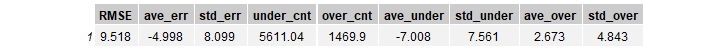
\includegraphics[width = \linewidth]{Control_tbl.png}
     \caption{Control Data Error Vector Summary}
     \label{fig:control_table}
 \end{figure}
 \begin{figure}
     \centering
     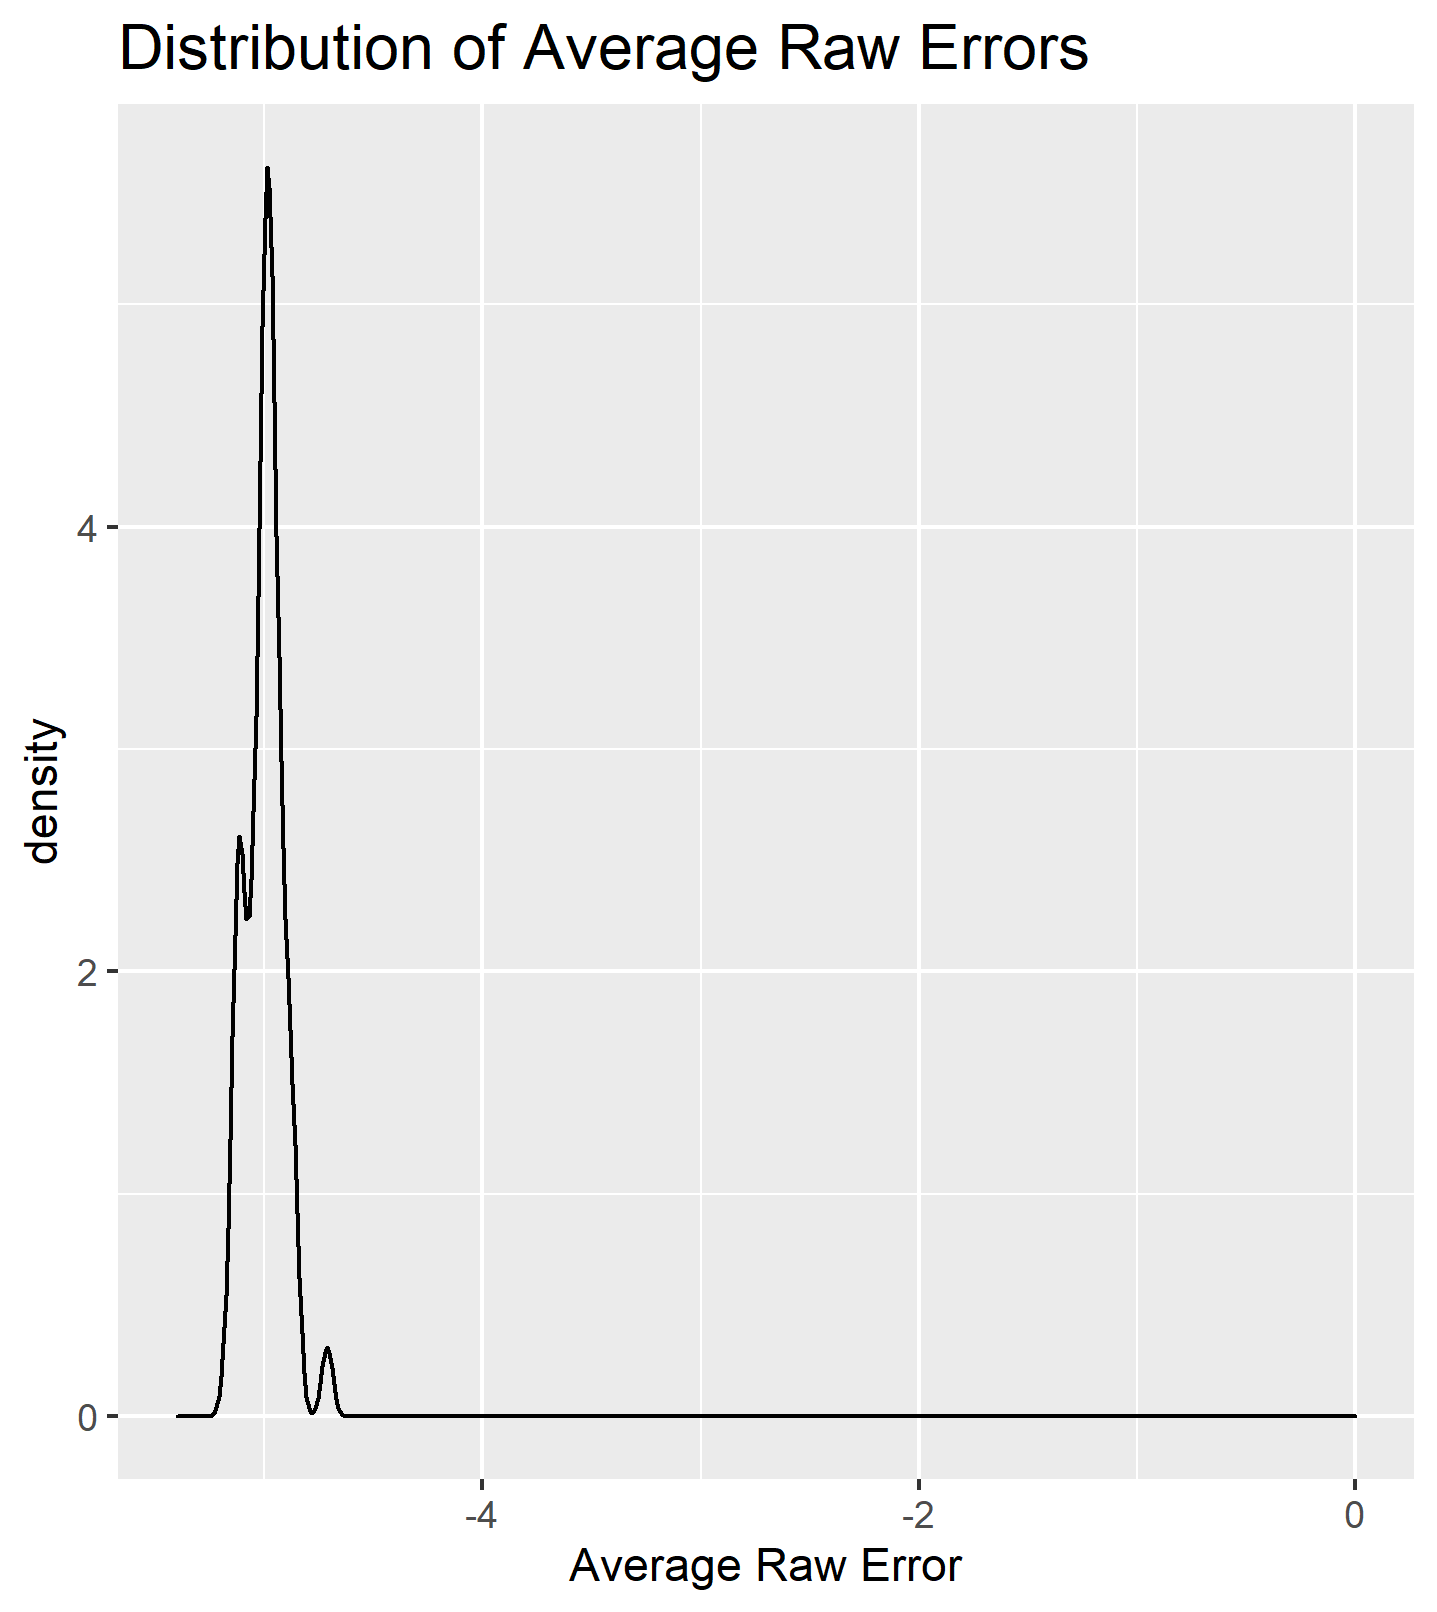
\includegraphics[width=0.35\linewidth]{control_ave_err_density.png}
     \caption{Density plot of raw error averages.}
     \label{fig:cntrl_ave_err}
 \end{figure}
  \end{frame}
  \begin{frame}{Results -- Control Data}
      \begin{figure}
          \centering
          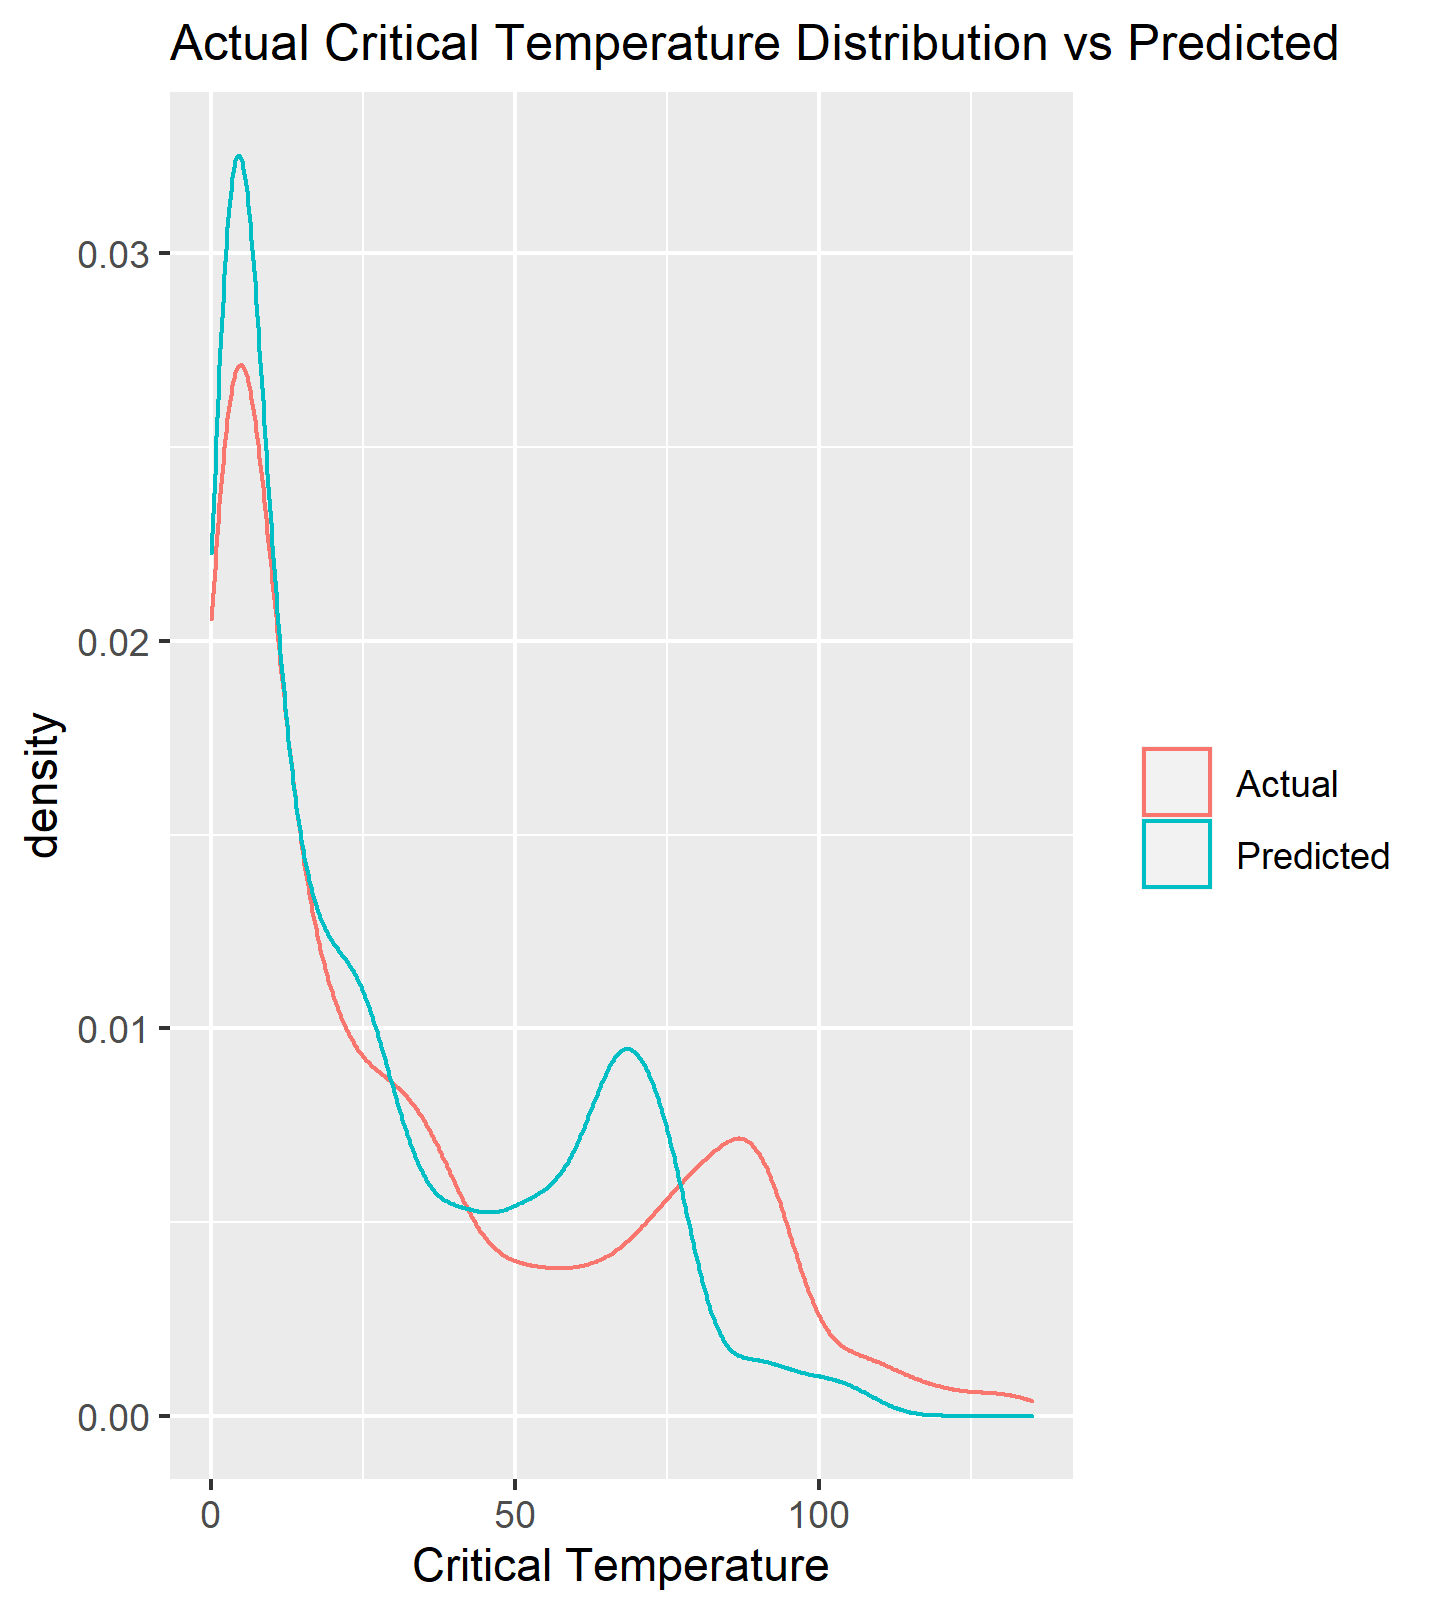
\includegraphics[width=0.5\linewidth]{Actual_vs_Pred_dist.png}
          \caption{Actual $T_c$ distribution plotted alongside predicted $T_c$ distribution.}
          \label{fig:comparsion_dist}
      \end{figure}
  \end{frame}
  
%   \begin{frame}{Results -- Element Subsets, No Retrain}
%   \begin{figure}
%       \centering
%       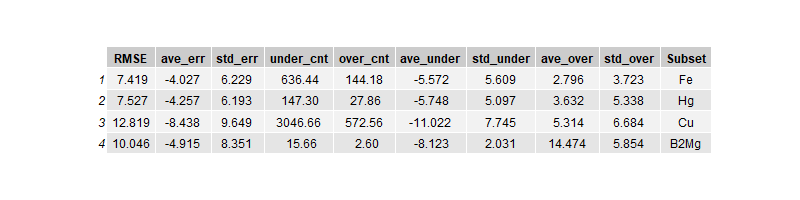
\includegraphics[width = \linewidth]{Elelmental_nrt_ave_tbl.png}
%       \caption{Average Error statistics for each element subset.}
%       \label{fig:ave_err_tbl_nrt_el}
%   \end{figure}
%   \end{frame}
%   \begin{frame}{Results -- Element Subsets, No Retrain}
%       \begin{figure}
%           \centering
%           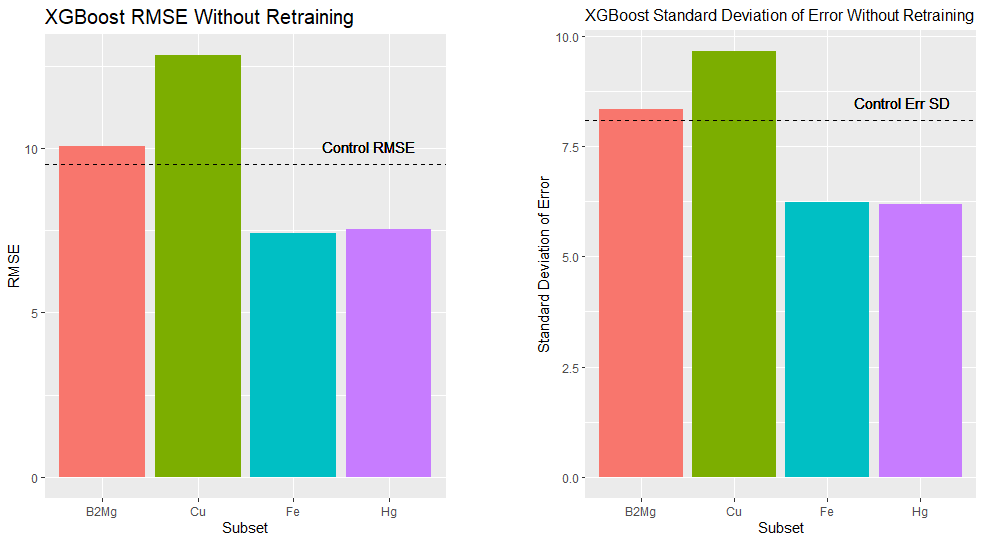
\includegraphics[width = 0.8\linewidth]{Elemental_nrt_bxplt.png}
%           \caption{RMSE and standard deviation of error for the element subsets with no retraining.}
%           \label{fig:nrt_el_brplt}
%       \end{figure}
%   \end{frame}
  
%   \begin{frame}{Results -- Element Subsets, With Retraining}
%       \begin{figure}
%           \centering
%           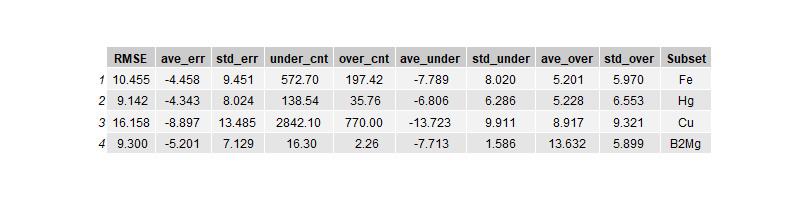
\includegraphics[width = \linewidth]{Elelmental_rt_ave_tbl.png}
%           \caption{Average Error statistics for each element subset with retraining}
%           \label{fig:el_ev_rt_tbl}
%       \end{figure}
%   \end{frame}
  
%   \begin{frame}{Results -- Element Subsets, With Retraining}
%       \begin{figure}
%           \centering
%           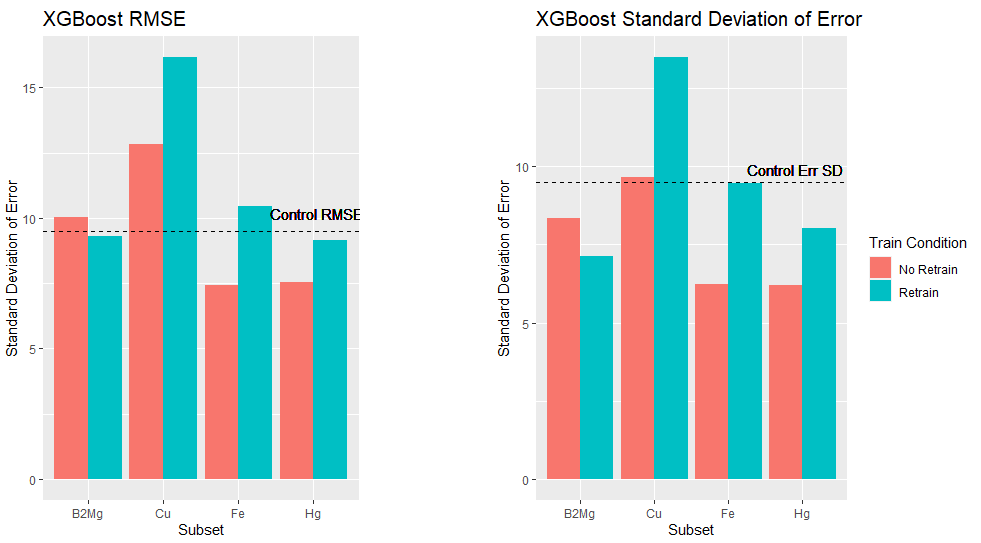
\includegraphics[width = 0.8\linewidth]{Elemental_comparison_bxplt.png}
%           \caption{Comparison of RMSE and standard deviation between retraining and no retraining conditions.}
%           \label{fig:el_cmp_rt_brplt}
%       \end{figure}
%   \end{frame}
  
%   \begin{frame}{Results -- True $T_c$ Quartiles}
%       \begin{figure}
%           \centering
%           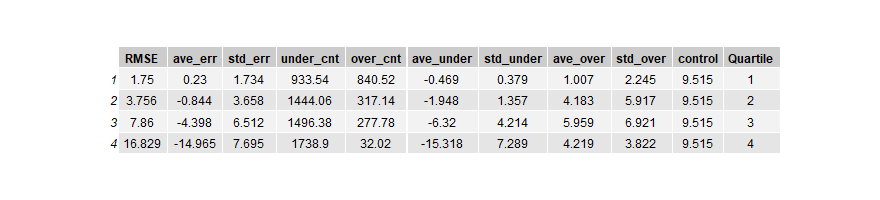
\includegraphics[width = \linewidth]{quart_true_ave_tbl.png}
%           \caption{Average error statistics for the true $T_c$ Quartiles}
%           \label{fig:tr_tc_q_tbl}
%       \end{figure}
%   \end{frame}
  \begin{frame}{Results -- True $T_c$ Quartiles}
    \begin{figure}
        \centering
        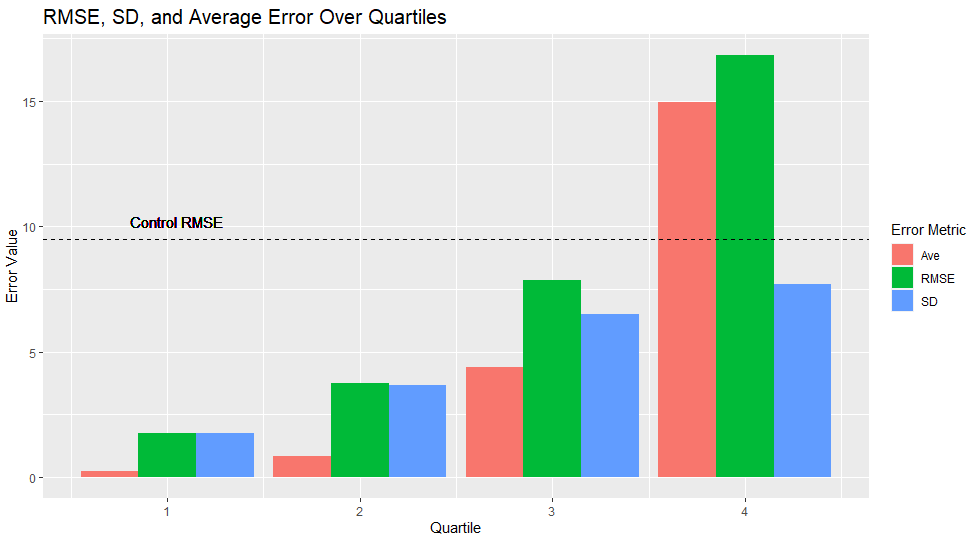
\includegraphics[width = 0.8\linewidth]{True_Q_Ave_brplt.png}
        \caption{RMSE, standard deviation of error, and the average of raw errors plotted alongside each other for each true $T_c$ quartile.}
        \label{fig:true_tc_q_brplt}
    \end{figure}
  \end{frame}
  
%   \begin{frame}{Results -- Predicted $T_c$ Quartiles}
%       \begin{figure}
%           \centering
%           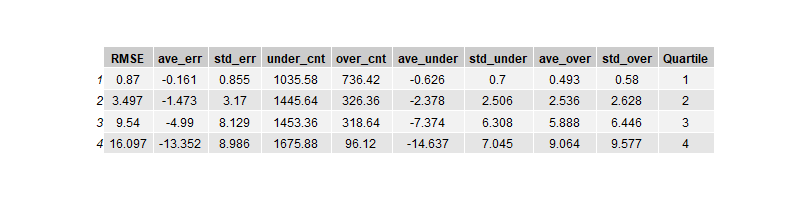
\includegraphics[width = \linewidth]{quart_pred_ave_tbl.png}
%           \caption{Average error statistics for the predicted $T_c$ Quartiles}
%           \label{fig:pred_tc_q_tbl}
%       \end{figure}
%   \end{frame}
  \begin{frame}{Results -- Predicted $T_c$ Quartiles}
      \begin{figure}
          \centering
          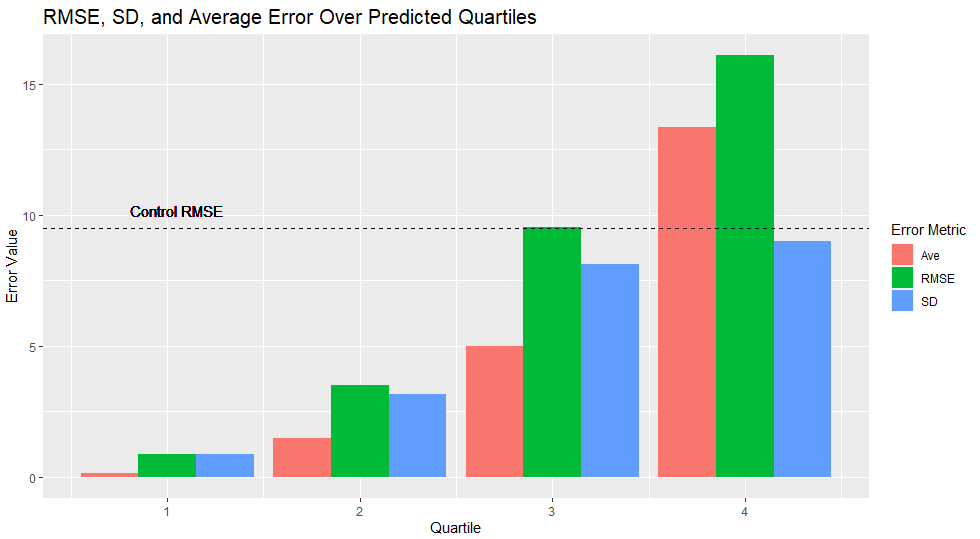
\includegraphics[width = 0.8\linewidth]{Pred_Q_Ave_brplt.png}
          \caption{RMSE, standard deviation of error, and the average of raw error plotted alongside each other for each predicted $T_c$ quartile.}
          \label{fig:pred_tc_q_brplt}
      \end{figure}
  \end{frame}
  
  \begin{frame}{Conclusion}
      \begin{block}{Summary}
        \begin{itemize}
            \item XGBoost performs with rapidly decreasing accuracy for increasing true $T_c$ quartiles.
            \begin{itemize}
                \item Largely due to correctable bias
            \end{itemize}
            \item XGBoost performs with rapidly decreasing accuracy for increasing predicted $T_c$ quartiles.
            \begin{itemize}
                \item Largely due to correctable bias
            \end{itemize}
        \end{itemize}
      \end{block}
  \end{frame}
  \begin{frame}{Conclusion}
      \begin{block}{Future Directions}
        \begin{itemize}
            \item Implementing corrections to XGBoost
            \begin{itemize}
                \item Via modified loss function
                \item Via additive correction term which depends on predicted quartile
            \end{itemize}
            \item Analysing distribution of raw errors without taking summary statistics 
        \end{itemize}
      \end{block}
  \end{frame}
\begin{frame}{References}
    \printbibliography
\end{frame}


\end{document}